\section{Automating Metadata Acquisition}

-building names dirty -> we need some way to characterize them
-learn
-input output example
-who will generate these - maybe building manager, maybe users
-ease of use as opposed to people writing regular expressoin themselves.
-why not have someone write the regex expressions for those most common sensors ? because people who know are not the people who use the data. building managers know, people working closely with a sensor deployment know. Sometimes the regex might get complex ...... for instanct, when is a particular tag applicable ? 

Why is it this way ?

In this section, we go into detail about how to extract sufficient information from sensor name to enable sufficient coverage of sensor applications. As explained earlier, most sensor names ( or SCADA\footnote{Supervisory Control and Data Acquisition} tags ) try to encode some level of semantic information. These names might have been generated by the individual who was in charge of commissioning a building, or by following a set of vendor-specific rules. A lot of the sense points contained in a particular building is very site-specific, e.g a building may contain a fault detector for its backup chiller, for which there might not be a well-defined sensor labelling schema from the vendor. In such scenarios, the agent commissioning a building tries his best to convey the information by using indicative labels. E.g we encountered points labelled \texttt{BLDA4S18SASA\_M}. However, these indicative labels might not be very illuminating to others

Most of these scada tags were generated by hand, and follows some pattern to make them discernable by the building-expert. These tags may include acronyms such as 'ARS' for the room setpoint temperature. Some of the information maybe encoded by simple letters such as a stra 'A1' indicating that the point is connected with an air handler, whose id is 1. This This renders it impossible to other tags may be 

some intro into what we are doing to automate



\subsection{final output - project Haystack}

final output maybe in any form. 
we realized going into this soon that not all tags conformed to any known schema. 
For the general tags like room, ahu, vav we have conformed to the project haystack ones. 
for the remainder of the points which are building specific, we just require that a person uses a consistent schema. 


Boosting the metadata can enable better usability across buildings. The question automatically becomes which metadata space to normalize to. There are many metadata schemes devised for representing all buildings. Some of them are too specific and require heavy lifting, and some of them are too simple and do not meet the criteria of being expressive enough for the necessary facets of a building. 


The goal is to normalize the existing metadata. 

\subsection{ formalize what we want as output from a string token}

what is the input ? 
well the input is 



- the model is we present the user an example to classify
- the expert goes in and classified every tag he knows in the building. he can see the list of tags in the building while doing so. 
- the user also tells us which position each string corresponds to 
- whether a value is a constant or a variable.

\subsection{techniques - learning from example}

There is a lot of related work in obtaining structured data from unstructured data formats. 

1. learning by example
2. data wrangler

-the core idea is to generate as many possible regular expressions as possible and then slowly refine our model as we get more and more examples.



\subsection{Technique Overview}

The synthesis technique is adapted from ~\cite{gulwani}, and tries to learn the regular expressions which 

of our technique is to provide building-specific experts the ability to come up with ur technique tried to learn the regular expression patterns that 
\subsection{learning by example}

-The basic structure of our technique is derived from gluwani.
-The goal is to 

Our proposed technique is derived from the synthesis technique developed in ~\cite{}. In this section, we provide an overview of the technique, and then we will introduce how we adapt this technique to our problem. 

At a very high level, the algorithm tries to compute all possible transformations that can transform an input string to an output string. The possibilities include a {\it Substring(i,j)} operation or simple position matching operation {\it{CPos}}. The two indices in the substring operation can be obtained by a regular expression, where the regular expression is  



 way we learn regular expressions from inputs provided by the expert. We shall use the example scada tag {\tt BLDA1R465  ART} as a goto example throughout this section.

In the following sections, we will use the word {\it token} to refer a token from a character class. So a token might be is a character or a group of characters in a point to be expanded. In the For instance, in the point {\tt BLDA1R465 ART} has the tokens as shown in Figure~\ref{fig:exampleInput}


\subsubsection{Inputs}

For every example an expert provides, we require three types of information - (a) the normalized metadata tag which is contained in the point name,  (b) the mapping of the labels in the data to normalized metadata tags , (c) the starting point of those labels, and (d) whether the value of the label is a constant or variable. For instance, consider the expert is asked to fully qualify the sensor point name \texttt{BLDA1R435\_\_ART}. Shown below is the expected input by the user.

\begin{figure}[h!]
  
  \centering
    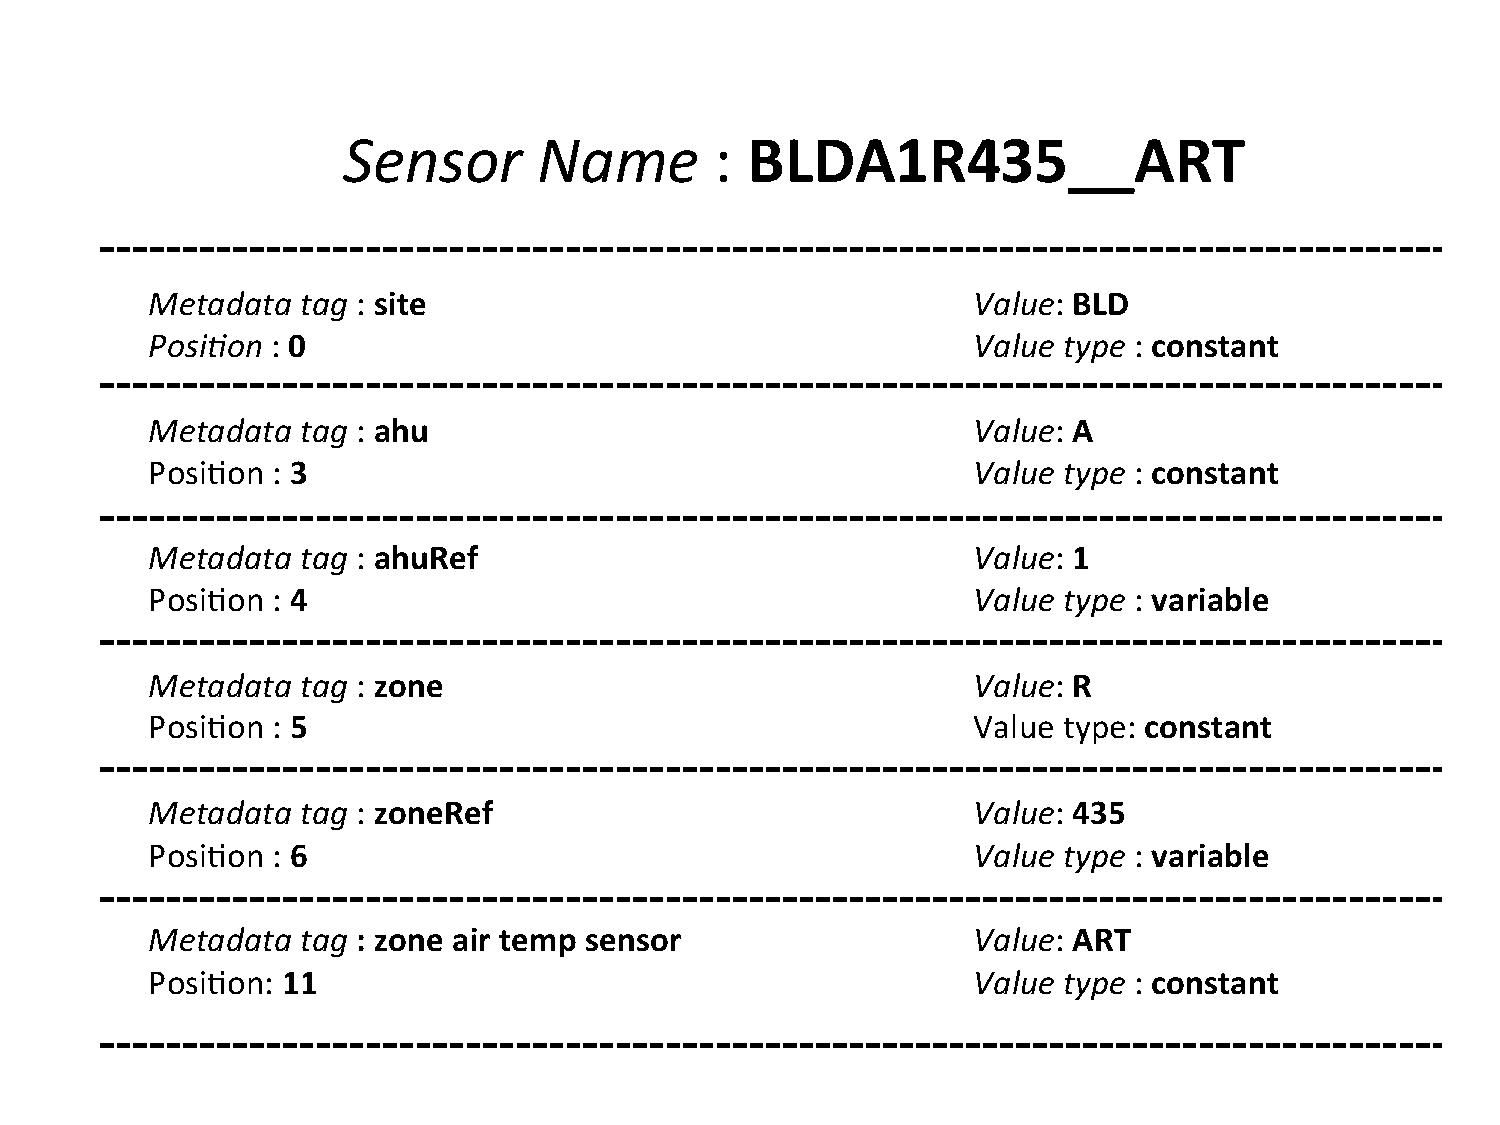
\includegraphics[width=0.5\textwidth]{figs/inputExample.pdf}
\caption{Input provided by the expert for fully qualifying the semantic structure of a sensor point name}
\label{fig:exampleInput}
\end{figure}

The aim of the learning algorithm would then be to fully qualify the remaining examples



Whenever the expert types in the explanation for an input, we require that the expert give a full description of the point. The full description of a point consist of the haystack tags the point contains, the starting and ending position of the string that correspond to the haystack tag, mentioning whether the substring is a constant or is variable. For instance, in our example, {\tt BLD} is a constant for the haystack tag {\bf site}, but {\tt 465} is a variable substring, because the tag value will change from point to point. 


are the tokens contained in a tag, their starting and ending positions, whether the tag has an associated value, and whether the associated value 

\subsection{challenges}


-different types of points all together in the same corpus, and it is not one or two . you have to generate a regex classifier for all known tags. 
-tokens vary from building to building -> so no pre-defined token ( alternative were using Excel's stuff or treating every letter as an individual token ). Show the experiment that shows the number of incorrectly qualified vs number of examples added.
-simplest classifier to more complex classifier



\subsection{technique we chose and modifications}

learning by input output example
- subtring generation
-intersection
-predicate generation


\subsection{Choosing Next Example for Expert}

Since the number of sensors in a building might be large ( more than 1000 sensors in some cases ), presenting an appropriate example to the expert for classification 
\begin{figure}[ht]
\centering
	\begin{subfigure}{0.48\textwidth}
                \centering
		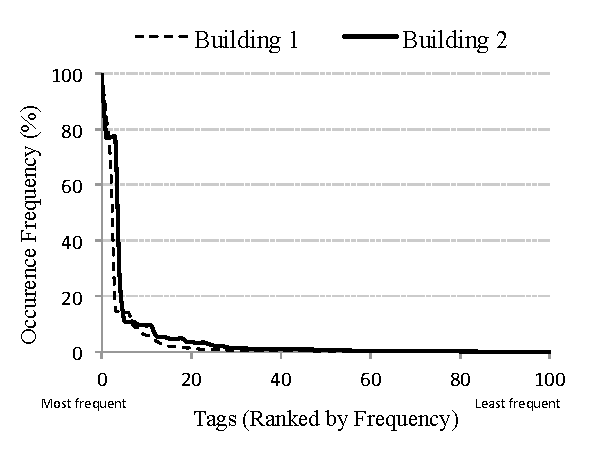
\includegraphics[width=\textwidth]{./figs/pointOccuranceFreq.pdf}
                \caption{Number of Points vs Year Built}
                \label{fig:sense_pts_data_yb}
	\end{subfigure}
	\begin{subfigure}{0.48\textwidth}
                \centering
		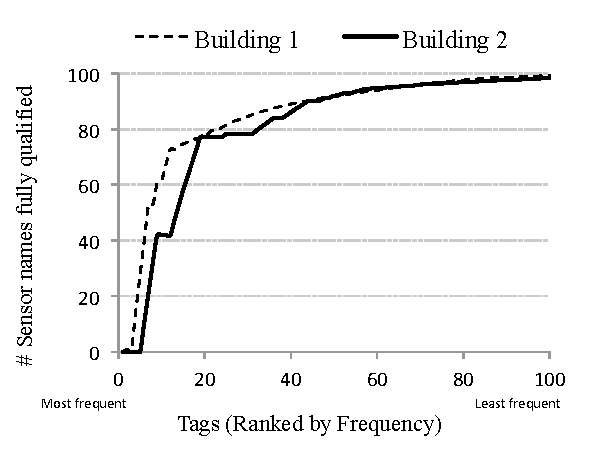
\includegraphics[width=\textwidth]{./figs/pointCDF}
                \caption{Number of Points vs Building Size}
                \label{fig:sense_pts_data_bs}
	\end{subfigure}
\caption{Relationship between the built year and the building size on the number of sense
points.  This data is summarize from a testbed that we used for experiments that consists of
almost 60 buildings and over 20,000 sense points.}
\label{fig:sense_pts_data}
\end{figure}

- min remaining
-max remaining 
-random run through the space.
Learning through input-output examples, though very intuitive to understand, and easy for a naive end-user faces several challenges. Unlike simple spreadsheet processing, a typical building may have multiple tokens  which 



2 pages




\subsection{applying to other buildings}







